\documentclass[12pt]{article}

\usepackage{fullpage}
\usepackage{multicol,multirow}
\usepackage{tabularx}
\usepackage{listings}
\usepackage{pgfplots}
\usepackage[utf8]{inputenc}
\usepackage[russian]{babel}

% Оригиналный шаблон: http://k806.ru/dalabs/da-report-template-2012.tex

\begin{document}

\section*{Лабораторная работа №1\, по курсу дискрeтного анализа: Сортировки за линейное время}

Выполнил студент группы М8О-212Б-22 МАИ \textit{Юрков Евгений}.

\subsection*{Условие}

\textbf{Вариант:} 7-1 

Требуется разработать программу, осуществляющую ввод пар «ключ-значение», их упорядочивание по возрастанию ключа
указанным алгоритмом сортировки за линейное время и вывод отсортированной последовательности.
Вариант задания определяется типом ключа (и соответствующим ему методом сортировки) и типом значения:
Поразрядная сортировка.

Тип ключа: автомобильные номера в формате A 999 BC (используются буквы латинского алфавита).

Тип значения: строки фиксированной длины 64 символа, во входных данных могут встретиться строки меньшей длины,
при этом строка дополняется до 64-х нулевыми символами, которые не выводятся на экран.

\newpage
\subsection*{Метод решения}

Для поразрядной сортировки строки происходит сортировка подсчетом массива пар ключ-значение. По очереди в функцию сортировки подсчетом передается
сортируемый индекс от большего к меньшему (от 7 до 0, так как строки фиксированной длины).
Для сортировки подсчетом создается массив \texttt{counter} содержащий количество повторений каждого символа на позиции \texttt{i}.
Далее происходит расстановка ключей вместе с соответствующими им значениями в отсортированном порядке в новом массиве \texttt{result}.
На последнем шаге происходит перемещение информации в исходный массив.

\newpage
\subsection*{Описание программы}

Данные хранятся в структуре \texttt{std::pair<std::string, std::string>}.
Программа состоит из следующих функций:
\begin{enumerate}
    \item \texttt{void \_\_count\_sort(std::vector<std::pair<std::string, std::string> >\& arr, uint index)}
    - функция осуществляющая сортировку подсчетом индекса \texttt{index} в массиве \texttt{arr}.
    \item \texttt{void radix\_sort(std::vector<std::pair<std::string, std::string> >\& arr)}
    - функция поразрядной сортировки для строки, сортирует значения строк в массиве передавая индексы в функцию сортировки подсчетом.
    \item \texttt{std::pair<std::string, std::string> parse(const std::string\& str)}
    - преобразует введенную строку в структуру ключ-значение.
    \item \texttt{int main()}.
\end{enumerate}

\newpage
\subsection*{Дневник отладки}

\begin{itemize}
    \item Сначала не были учтены пустые введенные строки и ключи без значений.
    \item Для преодоления ML во всех присваиваниях строк и массивов в функции сортировки подсчетом был использован \texttt{std::move( )}.
    \item Сначала использовалась поразрядная сортировка для чисел, но для преодоления TL функция сортировки была переписана специально для сортировки строк длины 8.
    \item Для сокращения времени перебора массива \texttt{counter} его размер был сокращен с 256 до \texttt{('Z' - '0' + 1)} 
    (теперь в нем храняться счетчики только тех символов, которые могут использоваться).
\end{itemize}

\newpage
\subsection*{Тест производительности}

Сложность написанного алогоритма $O(n)$. Для построения графика (Рис. 1) использовались тесты с 1 - 1000 строками данных.
Из графика видно, что количество входных данных слабо влияет на время работы программы.

\begin{figure}
    \centering
    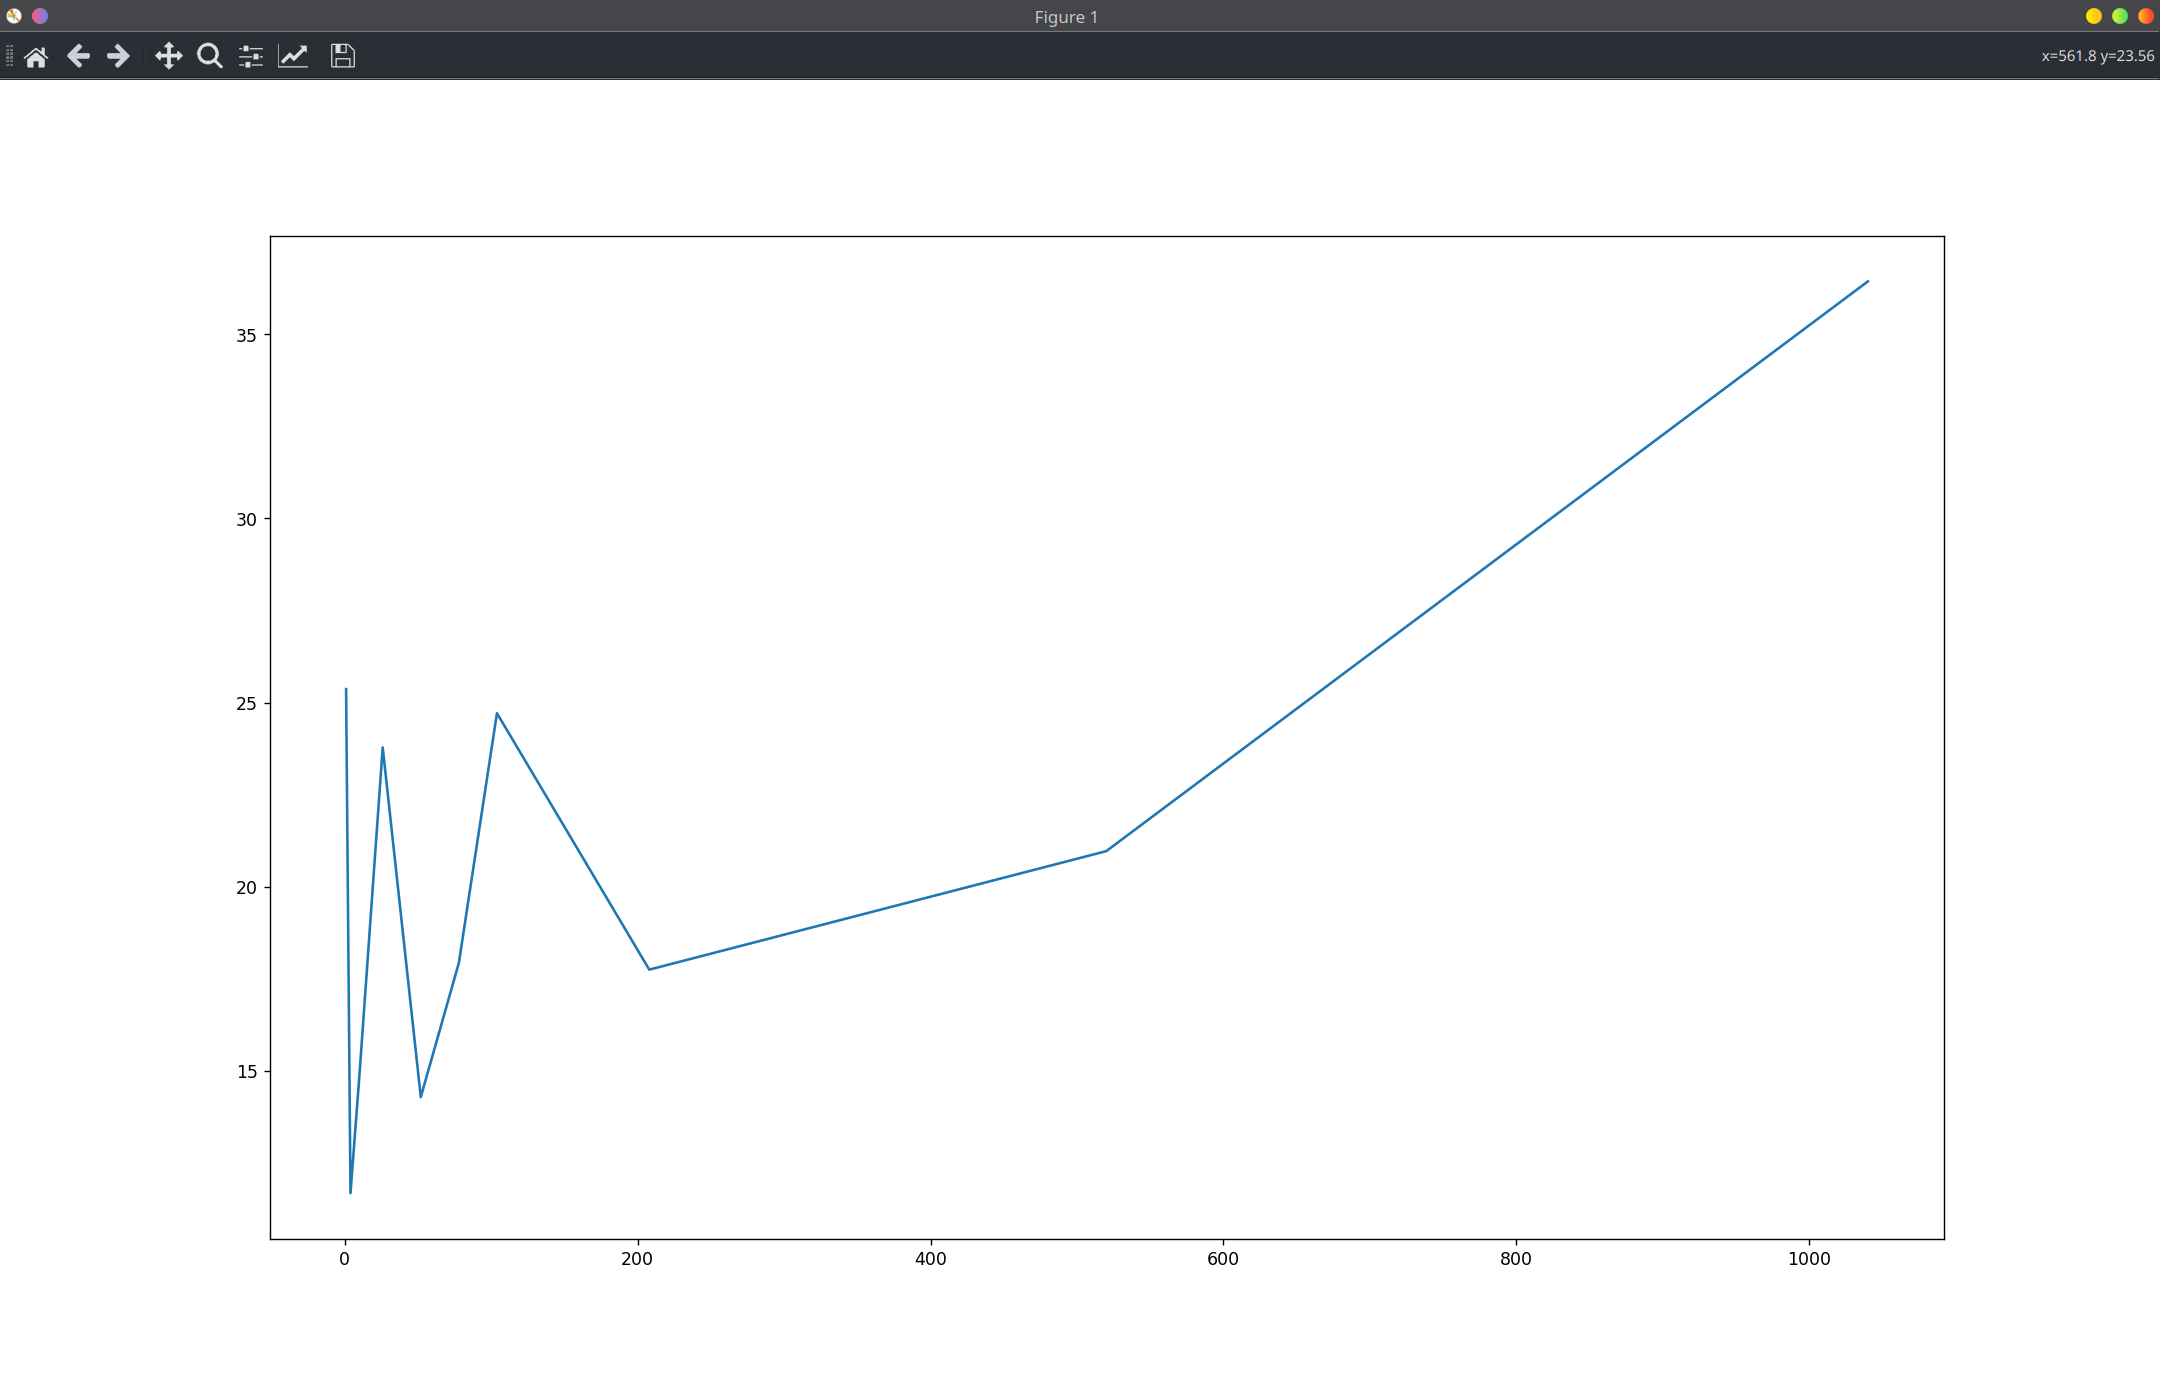
\includegraphics[width=\textwidth]{graph.png}
    \caption{График зависимости времени работы программы от количества введенных данных}
\end{figure}

\newpage
\subsection*{Выводы}

Поразрядная сортировка важна для эффективной обработки больших объемов данных, когда необходимо быстро выполнить сортировку.
Она позволяют обеспечить линейную сложность алгоритма относительно количества элементов в массиве,
что делает ее особенно полезной для больших и расширяющихся наборов данных.
Однако этот метод сортировки неприменим для сложных структур данных,
в этом он уступает сортировкам за $O(n \log n)$, для которых достаточно определить операцию сравнения элементов.

\end{document}
